\documentclass[border=10pt]{standalone}

\usepackage{tikz}

\begin{document}
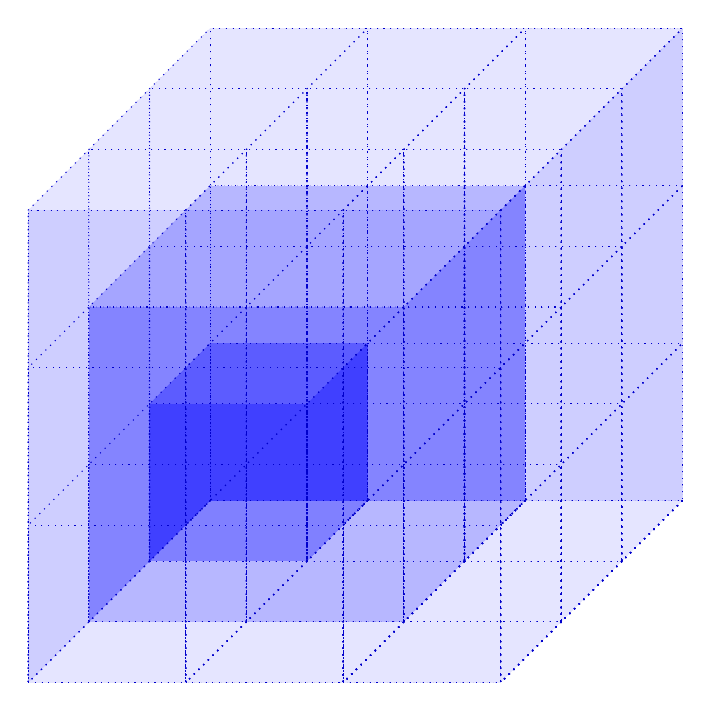
\begin{tikzpicture}[scale=2]
    % Largeset cube
    \fill[blue, opacity=.1, draw=blue!80!black, dotted] (0,0,0) -- (3,0,0) -- (3,3,0) -- (0,3,0) -- cycle;
    \fill[blue, opacity=.1, draw=blue!80!black, dotted] (0,0,0) -- (0,0,3) -- (0,3,3) -- (0,3,0);
    \fill[blue, opacity=.1, draw=blue!80!black, dotted] (3,0,0) -- (3,0,3) -- (3,3,3) -- (3,3,0);
    \fill[blue, opacity=.1, draw=blue!80!black, dotted] (0,0,3) -- (3,0,3) -- (3,3,3) -- (0,3,3) -- cycle;
    
    % Larger cube
    \fill[blue, opacity=.2, draw=blue!80!black, dotted] (0,0,0) -- (2,0,0) -- (2,2,0) -- (0,2,0) -- cycle;
    \fill[blue, opacity=.2, draw=blue!80!black, dotted] (0,0,0) -- (0,0,2) -- (0,2,2) -- (0,2,0);
    \fill[blue, opacity=.2, draw=blue!80!black, dotted] (2,0,0) -- (2,0,2) -- (2,2,2) -- (2,2,0);
    \fill[blue, opacity=.2, draw=blue!80!black, dotted] (0,0,2) -- (2,0,2) -- (2,2,2) -- (0,2,2) -- cycle;
    
    % Smaller cube
    \fill[blue, opacity=.3, draw=blue!80!black, dotted] (0,0,0) -- (1,0,0) -- (1,1,0) -- (0,1,0) -- cycle;
    \fill[blue, opacity=.3, draw=blue!80!black, dotted] (0,0,0) -- (0,0,1) -- (0,1,1) -- (0,1,0);
    \fill[blue, opacity=.3, draw=blue!80!black, dotted] (1,0,0) -- (1,0,1) -- (1,1,1) -- (1,1,0);
    \fill[blue, opacity=.3, draw=blue!80!black, dotted] (0,0,1) -- (1,0,1) -- (1,1,1) -- (0,1,1) -- cycle;

    % Smaller cube
    \foreach \x in {0,1,2} {
        \foreach \y in {0,1,2} {
            \foreach \z in {0,1,2} {
                \draw[blue!80!black, dotted] (\x,0,\z) -- (\x+1,0,\z) -- (\x+1,\y+1,\z) -- (\x,\y+1,\z) -- cycle;
                \draw[blue!80!black, dotted] (\x,0,\z) -- (\x,0,\z+1) -- (\x,\y+1,\z+1) -- (\x,\y+1,\z);
                \draw[blue!80!black, dotted] (\x+1,0,\z) -- (\x+1,0,\z+1) -- (\x+1,\y+1,\z+1) -- (\x+1,\y+1,\z);
                \draw[blue!80!black, dotted] (\x,0,\z+1) -- (\x+1,0,\z+1) -- (\x+1,\y+1,\z+1) -- (\x,\y+1,\z+1) -- cycle;
                % Smaller cube
                \draw[blue!80!black, dotted] (2,0,\z) -- (3,0,\z) -- (3,\y+1,\z) -- (2,\y+1,\z) -- cycle;
                \draw[blue!80!black, dotted] (2,0,\z) -- (2,0,\z+1) -- (2,\y+1,\z+1) -- (2,\y+1,\z);
                \draw[blue!80!black, dotted] (3,0,\z) -- (3,0,\z+1) -- (3,\y+1,\z+1) -- (3,\y+1,\z);
                \draw[blue!80!black, dotted] (2,0,\z+1) -- (3,0,\z+1) -- (3,\y+1,\z+1) -- (2,\y+1,\z+1) -- cycle;
            }
        }
    }
\end{tikzpicture}
\end{document}
